\documentclass[notitlepage]{report}
\usepackage{url}
\usepackage{hyperref}
\usepackage{graphicx}
\graphicspath{ {assets/} }
\usepackage{caption}

% Subtract 1 from counters that are used
\renewcommand{\thesection}{\number\numexpr\value{section}\relax}
\renewcommand{\thesubsection}{\thesection.\number\numexpr\value{subsection}\relax}
\renewcommand{\thesubsubsection}{\thesubsection.\number\numexpr\value{subsubsection}\relax}
\setcounter{secnumdepth}{3}
\setcounter{chapter}{1}
\renewcommand\thefigure{\arabic{figure}}
\setcounter{figure}{0}

\title{Monero v7 Mining Pool Report}
% \date{May 2018}
\author{sneurlax \\
\textless\url{sneurlax@gmail.com}\textgreater \\
(\url{https://github.com/sneurlax})}

\begin{document}
\maketitle
\thispagestyle{empty}

\section*{Abstract}

This is an overview of Monero version 7 mining pools with a current example of degraded privacy in one of Monero's privacy layers due to poor practices on the part of mining pools, a report on mitigation strategies including submissions to the blackball database, and a request for comments on best practices or solutions going forward.  This report applies to Monero mainnet version 7 (v7) and showcases degraded privacy due to publicly-available metadata: mining pools' announced finds (blocks) and payments (transactions.)  Mining pools are recommended to improve "privacy by obscurity" by disclosing less information publicly, but simple practices are presented in order to allow mining pools to proactively improve their privacy while maintaining their current level of metadata disclosure.

\clearpage

\tableofcontents

\section{Introduction}

\setcounter{page}{1}

As of Monero version 7 (\verb/v7/, which began at block height 1546000,\footnote{\href{https://github.com/monero-project/monero/blob/93e76e14a205a84cbea8ab0a3e35f37bf9d08b42/src/cryptonote_core/blockchain.cpp\#L111}{monero/src/cryptonote\_core/blockchain.cpp v0.12.0.0, line 111.}}) a majority of the Monero hashrate is attributable to particular mining pools and there are seven or eight public pools with over 1\% of the total global hashrate.\footnote{See section \ref{state-of-the-hashrate}.}  These pools advertise various statistics---metadata---including the blocks that they have mined, and all but one pool list the payouts that they have made to their miners.\footnote{See footnote \ref{nanopool-surprisingly-not-the-worst}.}  The combination of output ownership and transaction authorship allow the true member of some ring signatures to be inferred beyond a reasonable doubt in some cases, degrading one of Monero's layers of privacy.\footnote{See sections \ref{cause} and \ref{effect}.}

\subsection{Monero's privacy protections}

As of \verb/v7/, Monero provides stealth addresses, ring signatures, and Ring Confidential Transactions (RingCT) as privacy layers.  These layers ensure that Monero transactions are unlinkable, untraceable, and opaque.  Stealth addresses provide unlinkability by encrypting the recipients of payments such that only the recipient of a Monero transaction can detect it as addressed to them, ring signatures provide untraceability by concealing the source of a payment such that any one of a number of ring members should be equally-plausible as the actual source of a Monero transaction, and Ring Confidential Transactions provide opaqueness by encrypting a payment's input and output amounts such that a third party cannot discern anything related to a transaction's amounts other than that it did not create new coins.

\subsection{Degraded untraceability of ring signatures due poor mining pool practices} \label{cause}

Ring signatures should conceal the real source of a Monero transaction.  When constructing transactions, Monero selects a number of "decoys" with which it constructs a ring signature: there is no way to discern which ring member actually made the transaction without additional information.  Unfortunately, poor mining pool practices such as blockchain forks and metadata announcements can provide enough additional information to discern which ring member is the actual source of a transaction beyond a reasonable doubt.

Blockchain forks have the potential to degrade the untraceability of ring signatures when users reuse key images across forks without taking advantage of any of the countermeasures provided by Monero's \verb/v7/ upgrade.  Key images may be safely (at least privately) reused across blockchain forks if care is taken to construct identical rings on both sides of the fork (a process which is outside of the scope of this report but is described in detail \href{https://monero.stackexchange.com/questions/7826/how-can-individuals-safeguard-themselves-and-the-community-against-a-key-reusing}{here}.\footnote{"How can individuals safeguard themselves and the community against a key reusing fork?" https://monero.stackexchange.com/questions/7826/how-can-individuals-safeguard-themselves-and-the-community-against-a-key-reusing})  If users send funds on both sids of the fork without any such precautions, however, then they will inadvertently produce two rings that share only one member in common, thus identifying the common member as the real source of both transactions.  Such outputs are identified as "known spent."

Mining pools have also been inadvertently revealing the real source of some payments \textit{via} the statistics that they advertise before any blockchain forks incentivized key image reuse.  Mining pools openly announce which outputs are theirs when they announce the blocks that they have found.  When they later announce a transaction that uses one of their outputs as a ring signature member, it is most likely that their output is the real one and known spent.

By identifying an output as real in one transaction, its suitability as a decoy is degraded elsewhere, reducing the effective ring size of other users' ring signatures when included in rings after they are revealed to be known spent.

\subsection{Monero version 7's countermeasures against privacy degradations} \label{effect}

Several tools were provided by the Monero \verb/v7/ upgrade that allow users to avoid or mitigate both of the above potential degradations to their privacy.  For example, users can avoid including any known spent outputs in their own ring signatures by using what is known as the blackball database, which contains every known spent output.  This report presents additional submissions to the blackball database, including explanations of what metadata identifies the real member of a ring, where to collect it, and example code to scrape and analyze the metadata necessary for independent verification of these results.

\section{The State of the Hashrate} \label{state-of-the-hashrate}

As of \verb/v7/, a majority of the network hashrate is attributable to public mining pools.\footnote{See Figure \ref{fig:hashrate-distribution} from \url{http://minexmr.com/pools.html}; however, independent verification of this information is a topic for future work and is possible as long as mining pools publicly disclose either a reported hashrate or at least their found blocks.}  Nanopool, SupportXMR, mineXMR.com, Mining Pool Hub, F2Pool, MinerGate, DwarfPool, and MoneroHash (the top 8 public Monero pools in descending order of hashrate) represent over 80\% of the combined global hashrate.  They all announce enough information to discern some outputs as known spent.\footnote{All of the pools announce their finds (blocks) and all but one (Nanopool) list all of their payments (transactions.)  Nanopool does not directly announce all of their payments, but still announces enough information to identify some outputs as spent, as detailed in section \ref{Nanopool}.  What portion of their total payments are attributable is not known at this time and is a topic for future work. \label{nanopool-surprisingly-not-the-worst}}

\begin{figure}[h]
\centering
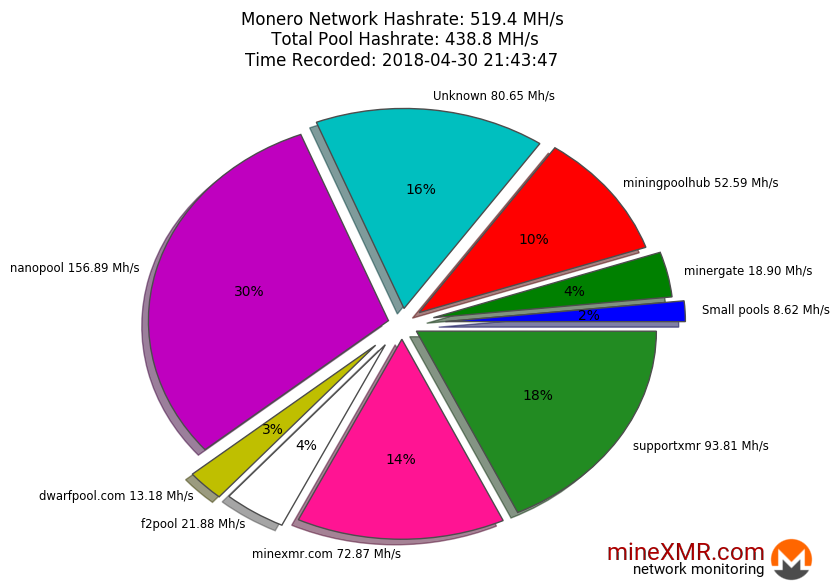
\includegraphics[width=\textwidth]{global-monero-mining-network-hashrate-distribution-2018-04-30}
\captionsetup{labelformat=empty}
\caption{Global Monero Mining Network Hashrate Distribution}
\label{fig:hashrate-distribution}
\end{figure}

\subsection{Software centralization}

TODO: List the most common mining pool stratum servers and GUIs and how code reuse enabled scraping of the data used to prepare this report.  \textit{Thanks, poolui!}

% TODO remake the chart above with overlays labelling distribution of software.

\section{Metadata collection}

TODO: Describe the metadata that will be collected, where it will be collected from, and how it will be used.

\subsection{poolui-format pools}

\subsection{Nanopool} \label{Nanopool}

\section{Mitigation}

TODO: Pool operators: either announce less information *or* churn prior to paying out to miners.

\subsection{Blackball database submissions}

TODO: Describe the https://xmreuse.daemon.network API for querying blackball database submissions

\section{Future work}

\section{Conclusion}

\section{References}

\end{document}
